\documentclass[11pt,a4paper]{article}
\usepackage{multirow}
\usepackage[utf8]{inputenc}
\usepackage[italian]{babel}
\usepackage[margin=2.5cm]{geometry}
\usepackage{graphicx}
\usepackage{amsmath}
\usepackage{hyperref}
\usepackage{float}
\usepackage{tikz}
\usetikzlibrary{automata, positioning, arrows.meta}
\usepackage{pgfplots}
\pgfplotsset{compat=1.18}
\usepackage{colortbl} 
\usepackage[table,xcdraw]{xcolor}
\usepackage{listings}
\usepackage{xcolor}
\lstdefinestyle{pystyle}{
    backgroundcolor=\color{backcolour},   
    commentstyle=\color{codegreen}\itshape,
    keywordstyle=\color{blue}\bfseries,
    numberstyle=\tiny\color{codegray},
    stringstyle=\color{codepurple},
    basicstyle=\ttfamily\footnotesize,
    breakatwhitespace=false,         
    breaklines=true,                 
    captionpos=b,                    
    keepspaces=true,                 
    numbers=left,                    
    numbersep=5pt,                  
    showspaces=false,                
    showstringspaces=false,
    showtabs=false,                  
    tabsize=4
}
\lstset{style=pystyle}
\usepackage{biblatex}
\addbibresource{bibliography.bib}
% Definizione colori per il codice sorgente
\definecolor{codegreen}{rgb}{0,0.6,0}
\definecolor{codegray}{rgb}{0.5,0.5,0.5}
\definecolor{codepurple}{rgb}{0.58,0,0.82}
\definecolor{backcolour}{rgb}{0.96,0.96,0.96}



\definecolor{linkcolor}{HTML}{0006b1}

\hypersetup{
    colorlinks=true,
    linkcolor=linkcolor,
    filecolor=transparent,      
    urlcolor=linkcolor,
    citecolor=linkcolor
    }

\title{\textbf{Applicazione di un algoritmo Ant Colony Optimization al problema del Capacitated Vehicle Routing Problem}}
\author{Marco Spampinato}
\date{}

\begin{document}

\maketitle

Link alla repository: \href{https://github.com/marcospampi/progetto-cvrp}{GitHub - Progetto CVRP}.

\section{Introduzione}
Il presente elaborato documenta il processo di sviluppo e analsi di un algoritmo della famiglia \textit{Ant Colony Optimization} per la risoluzione del \textit{Capacitated Vehicle Routing Problem} (CVRP), un classico problema di ottimizzazione NP-hard e generalizzazione del \textit{Traveling Salesman Problem} (TSP).

\vspace{0.3cm}
\noindent
L'algoritmo realizzato è basato su \textit{Applying the ANT System to the Vehicle Routing Problem} \cite{Bullnheimer},  il quale propone un primo elegante e estensivamente descritto algoritmo \textit{ACO} per la risoluzione del CVPR, estendendo l'algoritmo \textit{Ant System} con l'applicazione di 2-Opt\cite{doi:10.1287/opre.6.6.791}, al fine di eliminare archi sovrapposti nello stesso percorso, così da semplificare la soluzione e ridurne il costo.

\vspace{0.3cm}
\noindent
È stata inoltre adottata l'euristica \textit{MAX-MIN} \cite{STUTZLE2000889}, la quale limita il decadimento e la saturazione del feromone, infine è stata implementata la possibilità di eseguire l'algoritmo su più processori, come suggerito da \cite{polacchi}, riducendo i tempi di esecuzione.
\subsection{Capacitated Vehicle Routing Problem}

Il \textit{Capacitated Vehicle Routing Problem} (CVRP) è un problema di ottimizzazione combinatoria NP-hard che estende il classico problema del commesso viaggiatore (TSP), introducendo vincoli di capacità sulle risorse di trasporto.

Formalmente, il problema può essere modellato su un grafo completo $G = (V, E)$, dove:
\begin{itemize}
    \item $V = \{v_0, v_1, \dots, v_n\}$ è l'insieme dei nodi, in cui il nodo $v_0$ rappresenta il deposito centrale e i restanti nodi $V \setminus \{v_0\} = \{ v_1, \dots, v_n\}$ rappresentano i clienti.
    \item $E = \{(i,j) : i,j \in V\}$ è l'insieme degli archi o percorsi che collegano i nodi, a ciascuno dei quali è associato un costo di percorrenza $d_{ij}$ (es. distanza o tempo).
    \item Ogni cliente $v_i \in V \setminus \{v_0\}$ richiede una quantità di merce pari a $q_i > 0$.
    \item Presso il deposito è disponibile una flotta di $m$ veicoli identici, ciascuno avente una capacità massima di carico pari a $Q$.
\end{itemize}
\noindent
L'obiettivo del CVRP è determinare un insieme di percorsi a costo totale minimo tali per cui:
\begin{enumerate}
    \item Ogni cliente venga visitato esattamente una volta da un solo veicolo.
    \item Ogni percorso inizi e termini obbligatoriamente presso il deposito centrale ($v_0$).
    \item Per ciascun veicolo $k$, la somma delle richieste dei clienti serviti in quel viaggio non superi la capacità massima $Q$:
\end{enumerate}

\begin{equation}
\sum_{i \in k} q_{i} \le Q \space : \space \forall k \in \text{Veicoli}
\end{equation}

\noindent
In termini intuitivi, il problema consiste nel pianificare i percorsi di una flotta di furgoni per servire tutti i clienti sparsi sul territorio, minimizzando la strada totale percorsa ed evitando che un qualsiasi veicolo superi il proprio limite di carico massimo durante il tragitto.

\subsection{Ant Colony Optimization}

L'algoritmo realizzato appartiene alla famiglia \textit{Ant Colony Optimization} (ACO); si definisce pertanto bio-ispirato in quanto simula il comportamento euristico delle formiche nell'approvvigionamento di risorse. Tale comportamento è fortemente influenzato dal \textbf{deposito di feromone} lungo i percorsi praticati verso il nido da parte delle formiche che trasportano il cibo. Questa sostanza agisce analogamente a una \textbf{memoria collettiva} e decentralizzata, influenzando le altre formiche della colonia a seguire i tracciati con maggiore concentrazione, fino a giungere alla fonte.

\vspace{.3cm}
\noindent
Il feromone è infine soggetto a \textit{evaporazione}, ovvero una progressiva e naturale riduzione della sua concentrazione nel tempo. È stato osservato che le formiche scelgono generalmente i percorsi più brevi: ciò è dovuto al fatto che sui tracciati più lunghi il tempo di percorrenza maggiore permette una superiore evaporazione, mentre sui percorsi più corti il passaggio più frequente delle formiche tende a mantenere il feromone più \textit{concentrato}, creando un \textbf{meccanismo di rinforzo positivo}.

\section{Algoritmo realizzato}

L'algoritmo realizzato genera ad ogni iterazione un numero \(K\) di soluzioni pari al numero di formiche della colonia, tali soluzioni sono influenzate dalle euristiche di visibilità e feromone. Generate le \(K\) soluzioni, una seconda fase, detta di \textit{aggiornamento}, riduce la quantità di feromone globale lungo i percorsi tramite \textit{evaporazione}, mentre rinforza i percorsi scelti dalle \(K\) soluzioni. L'algoritmo restituisce sempre la soluzione migliore trovata. 
\\Generalmente, \(K\) è fissato al numero di clienti nel problema. La \autoref{aco_pseudocode} mostra lo pseudocodice del ciclo principale dell'algoritmo.


\begin{figure}[H]
  \caption{Pseudocodice algoritmo ACO}
  \label{aco_pseudocode}
\begin{lstlisting}[gobble=2]
    while not terminated:
        generate K solutions
        store the best solution, if found
        update pheromone
    return best solution
        
\end{lstlisting}
\end{figure}
\noindent


\vspace{.3cm}
\subsection{Generazione delle soluzioni}
Ogni formica virtuale genera una soluzione visitando tutti i nodi cliente, in particolare la formica è definita dal seguente stato:
\begin{itemize}
    \item Una determinata posizione \(V_i\) ad ogni iterazione.
    \item Un carico \(Q_i\), corrispondente al carico residuo al nodo \(V_i\), dove vale sempre \(Q_{depot} = Q_{start} = Q\), data \(Q\) la capacità o carico massimo definito dell'istanza di problema .
    \item Una memoria dell'insieme dei nodi da visitare $\Omega$.
    \item Una memoria della lista dei percorsi, che chiameremo \textit{mini-tour}.
\end{itemize}

\vspace{.3cm}
\noindent
Come esemplificato in \autoref{ant_pseudocode}, ogni formica avvia l'esplorazione partendo da un certo nodo iniziale \(V_{start}\) e un \textit{mini-tour} vuoto; finché vi sono nodi non visitati ( ad eccezione del nodo di partenza e il deposito ), essa seleziona il prossimo nodo \(V_j\) tra i nodi non visitati, secondo una certa probabilità \(P_{ij}\). Qualora la domanda del nodo \(V_j\) superasse il carico \(Q_i\) della formica, la formica torna al deposito, resetta il suo carico a \(Q\) e inizia un nuovo \textit{mini-tour}; altrimenti visita il nodo \(V_j\), diminuendo il suo carico della domanda del nodo visitato, e aggiungendo \(V_j\) al \textit{mini-tour}.
\begin{figure}[H]
  \caption{Pseudocodice generazione di una soluzione}
  \label{ant_pseudocode}
\begin{lstlisting}[gobble=2]
    unvisited_nodes = all_nodes \ { Vdepot, Vstart }
    if Vstart != Vdepot: visit Vstart
    while |unvisited_nodes| > 0:
        select unvisited node Vj according to probability Pij
        if Vj's demand > load:
            visit depot and restore load
        else:
            unvisited_nodes = unvisited_nodes \ {Vj}
            visit node Vj and unload Vj's demand
    visit depot
    return solution
\end{lstlisting}
\end{figure}
\noindent
Vi sono tre strategie per scegliere \(V_{start}\):
\begin{itemize}
    \item Usare come punto di partenza il deposito: \(V_{start}=V_{depot}\).
    \item Assegnare il punto di partenza di ogni formica a un cliente \(V_{start}=V_{k}\).
    \item Usare un nodo random \(V_{start}=V_{rand()}\).
\end{itemize}
In letteratura, è stato sperimentalmente documentato che assegnare a ogni cliente una formica, determina un risultato di maggiore qualità.

\subsubsection{Scelta dei nodi da visitare}
La scelta del prossimo nodo da visitare è data dalla seguente distribuzione di probabilità:

\[
P_{ij} = 
\begin{cases} 
\frac{[\tau_{ij}]^\alpha \cdot [\eta_{ij}]^\beta}{\sum_{h \in \Omega} [\tau_{ih}]^\alpha \cdot [\eta_{ih}]^\beta} & \text{se } j \in \Omega \\ 
0 & \text{se } j \notin \Omega 
\end{cases}
\]
Dove:
\begin{itemize}
    \item \(\tau_{ij}\) è la quantità di feromone presente nell'arco \((i,j)\).
    \item \(\eta_{ij}\) è la costante di visibilità, inversamente proporzionale alla distanza tra \(V_{i}\) e \(V_{J}\), i.e. \(\eta_{ij}=d_{ij}^{-1}\).
    \item \(\alpha\) e \(\beta\) sono costanti che influenzano rispettivamente la scelta tra feromone e visibilità, ovvero pesano la scelta tra  \(P_{ij} \sim \tau_{ij}\) e \(P_{ij} \sim\eta_{ij}\).
    \item \(\Omega\) è l'insieme dei nodi non ancora visitati.
\end{itemize}

Al fine di migliorare la qualità dell'algoritmo, sono state adottate altre due euristiche usate in \cite{Bullnheimer}, le misure di \textit{risparmio} e \textit{capacità}, pertanto la effettiva probabilità realizzata è:
\[
P_{ij} = 
\begin{cases} 
\frac{[\tau_{ij}]^\alpha \cdot [\eta_{ij}]^\beta \cdot [\mu_{ij}]^\gamma \cdot [\kappa_{ij}]^\lambda}{\sum_{h \in \Omega} [\tau_{ih}]^\alpha \cdot [\eta_{ih}]^\beta\cdot [\mu_{ih}]^\gamma \cdot [\kappa_{ih}]^\lambda} & \text{se } j \in \Omega \\ 
0 & \text{se } j \notin \Omega 
\end{cases}
\]
Le due nuove euristiche sono:
\begin{itemize}
    \item La misura di \textit{risparmio} \(\mu_{ij}=d_{i0} + d_{0j} - d_{ij}\) quantifica quanto è conveniente visitare un nodo \(V_j\) dopo aver visitato \(V_i\), basandosi sulla distanza, è influenzata dall'esponente \(\gamma\).
    \item La misura di \textit{capacità} \(\kappa_{ij}=1-\frac{Q_i-q_j}{Q}\) quantifica quanto è conveniente visitare un nodo \(V_j\) basandosi su quanto carico \(Q_i\) ho ancora disponibile. Si precisa che la formulazione differisce da \cite{Bullnheimer}, in quanto il nostro algoritmo usa come metrica il carico residuo, anziché la capacità residua. Inoltre per \(k_{ij} > 1\), la soluzione è \textit{unfeasable}, ovvero non è possibile soddisfare la richiesta. 
\end{itemize}
\subsubsection{Soluzione finale}
Una volta visitati tutti i nodi, la formica virtuale costruisce una soluzione comprendente di:
\begin{itemize}
    \item Costo totale della soluzione, intesa come lunghezza complessiva di tutti i mini-tour.
    \item Un insieme di tutti i mini-tour appartenti alla soluzione.
\end{itemize}
Al fine di migliorare il risultato, come proposto in \cite{Bullnheimer}, è possibile eseguire sui mini-tour l'algoritmo \textit{2-Opt}, una euristica di ricerca locale che migliora un percorso eliminando due collegamenti e invertendo la tratta racchiusa, al fine di eliminare gli incroci e quindi ridurne la lunghezza.


\subsection{Aggiornamento del feromone}
Il feromone, una volta generate le \(K\) soluzioni, viene aggiornato dalla seguente formula:

\[
\tau_{ij} \xleftarrow{} (1-\rho)\cdot\tau_{ij} + \Delta\tau^{(S)}_{ij} + \sigma\Delta{\tau^\star_{ij}}
\]
Dove:
\begin{itemize}
    \item \(\rho\) è il coefficiente di evaporazione, regola quanto feromone viene perso in ogni iterazione
    \item \(\Delta\tau^{(S)}_{ij}\) è il deposito di feromone dipendente dalle soluzioni generate nella stessa generazione, vi sono state realizzate due strategie di aggiornamento:
    \begin{itemize}
        \item Deposito usando solo i percorsi usati dalla soluzione migliore della iterazione, questa strategia è generalmente la migliore.
        \item Deposito usando i percorsi realizzati da tutte le soluzioni.
    \end{itemize}
\item \(\sigma\Delta{\tau^\star_{ij}}\) è invece un contributo della migliore soluzione trovata, in letteratura prende il nome di \textit{formiche elitiste}, e simula il deposito di \(\sigma\) formiche usando la soluzione migliore globale. Solitamente \(\sigma = K\).
\end{itemize}

\subsubsection{MAX-MIN Ant System}
Da \cite{STUTZLE2000889}, MAX-MIN è una euristica atta a limitare il decadimento e l'accumulo del feromone, restringendo dunque i valori della matrice dei feromoni all'interno di un determianto range, rendendo più stabili i calcoli e favorendo una maggiore esplorazione dello spazio delle soluzioni.
\noindent
L'articolo originale propone un metodo per definire $\tau_{max}$ e $\tau_{min}$, tuttavia la formulazione di quest'ultimo è alquanto ostica, pertanto una sua semplificazione viene adottata.
\[
\tau_{max} = \frac{1}{\rho \cdot C^\star },\quad \tau_{min} = \frac{\tau_{max}}{2\cdot K}
\]
\noindent
Dove \(C^\star\) è la soluzione migliore globale. \textit{MAX-MIN} viene applicato successivamente l'aggiornamento dei feromoni.

\vspace{0.3cm}
\noindent
Una opzione non esplorata nell'analisi dei risultati, è lo \textit{smussamento} o \textit{smoothing}, una operazione di normalizzazione, che tende ad appiattire i livelli di feromoni secondo un parametro $\delta \in [0,1] $:
\[
\tau_{ij} \xleftarrow{} \tau_{ij} + \delta\cdot(\tau_{max}-\tau_{ij})
\]

\section{Implementazione}
L'algoritmo è stato implementato nel linguaggio di programmazione Python, facendo uso della libreria \textit{numpy} per varie utilità matematiche. Le classi e script prodotti sono:
\begin{itemize}
    \item La classe \texttt{Instance} cui responsabilità sono il caricamento dei file di istanza del problema in formato \texttt{.vrp}.
    \item La classe \texttt{Solution} che descrive una soluzione del problema, con funzionalità di verifica e serializzazione del soluzione.
    \item La classe astratta \texttt{BaseSolver}, la quale definisce una interfaccia comune ai vari algoritmi di risoluzione implementabili.
    \item La classe \texttt{ACOSolver}, la quale eredita \texttt{BaseSolver}, implementa l'algoritmo ACO come descritto precedentemente.
    \item La classe \texttt{ACO\_MPSolver}, estensione di \texttt{ACOSolver}, in grado di eseguire su più core l'algoritmo.
    \item Lo script \texttt{grinder.py}, il quale contiene il programma di automazione per eseguire l'algoritmo su diverse istanze e diversi profili di parametri.
    \item Lo script \texttt{utils.py} che contiene diverse utilità, tra cui la possibilità di stampare a video l'istanza di un problema e una sua soluzione.
    \item Gli script \texttt{main.py} e \texttt{grind.py}, i quali forniscono un accesso da riga di comando all'implementazione. 
\end{itemize}
Per maggiori informazioni, si invita a consultare il \textit{readme} dei sorgenti forniti.
\subsection{Stabilità numerica}
Uno dei problemi implementativi affrontati è stato quello della stabilità numerica: calcolare la probabilità \(P_{ij}\) al fine di selezionare un nodo da visitare, ha portato a diversi errori di runtime, quali \textit{underflow} e \textit{overflow}, dovuti ai limiti di precisione in virgola mobile.
\\Una operazione comune nel machine learning è la normalizzazione di probabilità in scala logaritmica, come il softmax:
\[
p_{i} = \frac{\exp(x_i)}{\sum_{n=1}^{N} \exp(x_n)} \qquad t.c. \space \sum_{i=1}^N p(x_i)=1
\]
Tale operazione nell'atto pratico è risolta calcolando il logaritmo di tale probabilità:
\[
p_i = \exp(\space x_i - \log(\sum_{n=1}^{N} \exp(x_n))\space) = \exp(\space x_i - LSE(x_1 ... x_n)\space)
\]
Ciò garantisce che  \(\max(p_i) \le \exp(0) = 1   \) e \(\sum_{n=1}^N p_i = 1\) senza problemi di stabilità numerica. Questa strategia matematica prende il nome di \textbf{Log-Sum-Exp trick}\cite{gundersen2020logsumexp}, ed è stata adottata per risolvere l'analogo calcolo di \(P_{ij}\).
\\In particolare possiamo scrivere:
\[
P_{ij} = 
\exp\begin{cases} 
\log\frac{[\tau_{ij}]^\alpha \cdot [\eta_{ij}]^\beta}{\sum_{l \in \Omega} [\tau_{il}]^\alpha \cdot [\eta_{il}]^\beta} & \text{se } j \in \Omega \\ 
-\infty & \text{se } j \notin \Omega 
\end{cases}
\]
E ricondurci a quanto visto prima:
\[
x_{ij} = \log([\tau_{ij}]^\alpha \cdot [\eta_{ij}]^\beta) = \alpha \cdot\log{\tau_{ij}} + \beta \cdot\log{\eta_{ij}}
\]
\[
P_{ij} = 
\exp\begin{cases} 
\log\frac{\exp(x_{ij})}{\sum_{h \in \Omega} {\exp(x_{ih})}} & \text{se } j \in \Omega \\ 
-\infty & \text{se } j \notin \Omega 
\end{cases}
\]
\[
P_{ij} = 
\begin{cases} 
\exp(x_{ij} - LSE(x_{i1}...x_{ih})) & \text{se } j \in \Omega  \\
0 & \text{se } j \notin \Omega 
\end{cases}
\]
\subsection{Computazione parallela}
La classe \textit{ACO\_MPSolver} implementa una specializzazione dell'algoritmo base in grado di eseguire il calcolo su più core, usando la libreria \textit{multiprocessing} e la sua classe \textit{Pool}, quale mette a disposizione un sistema per l'invocazione da parte dell'utente di funzioni Python su processi fork.
\\La classe sovrascrive il metodo della classe padre \textit{ACOSolver} responsabile della simulazione e generazione risultati, affinché il carico possa essere distribuito in blocchi su più processori usando la classe \textit{Pool}, riducendo significativamente i tempi di iterazione. 
\section{Sperimentazione e risultati}
L'algoritmo è stato testato su diverse istanze di problema assegnate dal docente. Ogni istanza è stata valutata su 7 differenti profili di parametri dell'algoritmo, e ogni profilo è stato valutato 5 volte sulla istanza data. Il criterio di terminazione assegnato è il numero di valutazioni della funzione fitness \(FE=3.5\cdot10^{5}\), poiché l'algoritmo computa \(K = numero\space clienti\) soluzioni ogni iterazione, il numero di iterazioni massime per istanza allora è pari a \(N = \lceil\frac{FE}{K}\rceil = \lceil\frac{3.5\cdot10^5}{K}\rceil \).

\begin{table}[h]
    \centering


    \begin{tabular}{|c||c|c|c|c|}\hline
  \textbf{Profilo} & \textbf{$\alpha$} & \textbf{$\beta$} & \textbf{$\gamma$} & \textbf{$\lambda$} \\\hline
          NN&  0&  1&  0&   0\\\hline
          AS&  1&  5&  0&   0\\\hline
          HAS&  1&  5&  0&   0\\\hline
          HAS-SAV&  1&  5&  5&   0\\\hline
          HAS-CAP&  1&  5&  0&   5\\\hline
          HAS-1&  1&  5&  5&   5\\ \hline
          HAS-5&  5&  5&  5&   5\\ \hline
    \end{tabular}
\caption{Profili utilizzati}
\label{tab:profiles}
    
    
\end{table}

\noindent
I profili usati derivano da \cite{Bullnheimer}. In particolare il profilo \textit{NN} corrisponde a una ricerca completamente stocastica, come nearest neightbour, infatti non vi è influenza del feromone. I profili della classe \textit{AS} e \textit{HAS} invece sono gli algoritmi ACO o \textit{Ant System}, dal nome originale dei primi algoritmi, e sono influenzati del feromone, gli algoritmi \textit{HAS} (\textit{Hybrid Ant System}) si contraddistinguono per eseguire \textit{2-Opt} su ogni mini-tour. Per tutti i profili, ad eccezione di \textit{NN}, è stato usato un numero \(\sigma=K\) di formiche elitarie e costante di evaporazione pari a \(\rho=0.25\), il deposito di feromone è stato consentito solo alle soluzioni migliori della iterazione, e infine è stato usato il \textit{MAX-MIN} per limitare la matrice dei feromoni \(\tau\).


\begin{table}[h]
\centering
\begin{tabular}{|l|l|l|l|l|l|l|l|}
\hline
\rowcolor[HTML]{EFEFEF} 
{\color[HTML]{343434} \textbf{Instanza}} & {\color[HTML]{343434} \textbf{Profilo}} & {\color[HTML]{343434} \textbf{KBS}} & {\color[HTML]{343434} \textbf{Best}} & {\color[HTML]{343434} \textbf{Err \%}} & {\color[HTML]{343434} \textbf{Media}} & {\color[HTML]{343434} \textbf{Std}} & {\color[HTML]{343434} \textbf{Avg. It.}} \\ \hline
A-n45-k7                        & HAS                                     & 1146.0                              & 1175.6                               & 2.583\%                                & 1181.86                               & 5.62                                & 5843.2                                   \\ \hline
\rowcolor[HTML]{ECF4FF} 
\textbf{A-n60-k9}                        & \textbf{HAS-5}                          & \textbf{1354.0}                     & \textbf{1372.94}                     & \textbf{1.399\%}                       & 1394.51                               & 17.97                               & 3580.6                                   \\ \hline
A-n80-k10                       & AS                                      & 1763.0                              & 1824.06                              & 3.463\%                                & 1839.3                                & 15.81                               & 2704.6                                   \\ \hline
\rowcolor[HTML]{ECF4FF} 
B-n56-k7                        & HAS-5                                   & 707.0                               & 755.62                               & 6.877\%                                & 764.78                                & 8.8                                 & 3663.6                                   \\ \hline
\textbf{B-n66-k9}                        & \textbf{AS}                             & \textbf{1316.0}                     & \textbf{1338.72}                     & \textbf{1.726\%}                       & \textbf{1341.88}                      & \textbf{2.38}                       & 2954.0                                   \\ \hline
B-n78-k10                       & HAS-5                                   & 1221.0                              & 1273.12                              & 4.269\%                                & 1283.98                               & 9.99                                & 2495.0                                   \\ \hline
\rowcolor[HTML]{ECF4FF} 
E-n101-k14                      & HAS-SAV                                 & 1071.0                              & 1141.05                              & 6.540\%                                & 1151.89                               & 8.94                                & 2621.6                                   \\ \hline
E-n76-k8                        & HAS-1                                   & 735.0                               & 758.97                               & 3.261\%                                & 771.25                                & 10.78                               & 3369.8                                   \\ \hline
P-n101-k4                       & HAS-1                                   & 681.0                               & 697.04                               & 2.356\%                                & 705.09                                & 4.84                                & 2021.8                                   \\ \hline
\textbf{P-n50-k10}                       & \textbf{HAS-5}                          & \textbf{696.0}                      & \textbf{707.03}                      & \textbf{1.585\%}                       & \textbf{720.84}                       & 10.26                               & 1506.2                                   \\ \hline
\end{tabular}
\caption{Risultati migliori. In grassetto i risultati più importanti.}
\label{tab:best_results}
\end{table}
\begin{figure}[H]
    \centering
    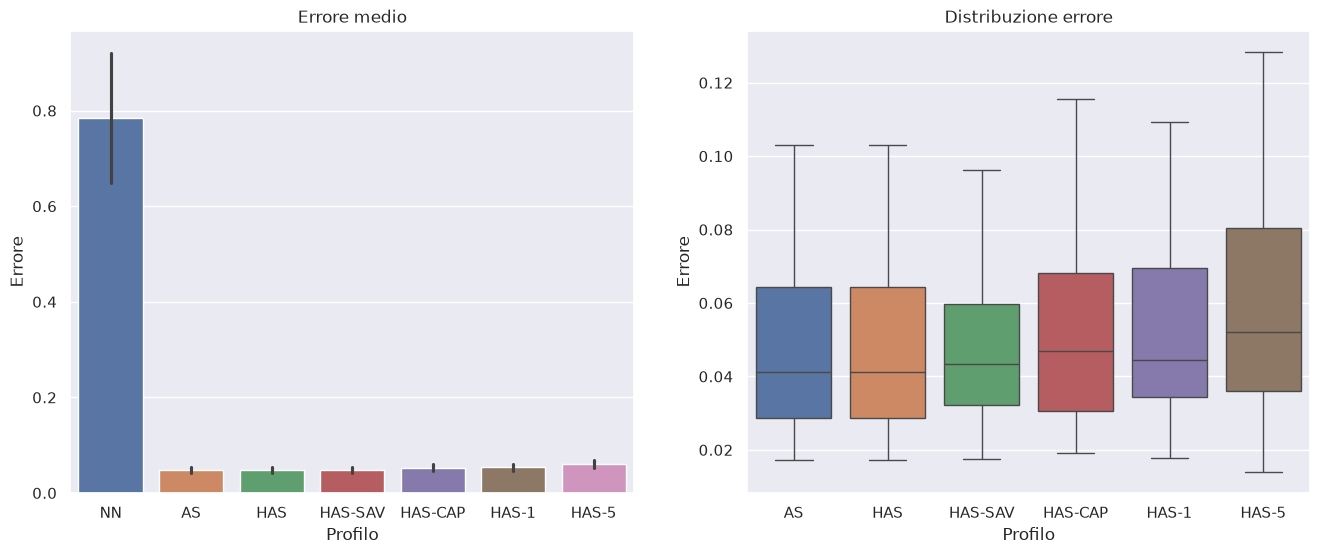
\includegraphics[width=1\linewidth]{error.png}
    \caption{Errore medio e distribuzione per profilo.}
    \label{fig:error}
\end{figure}
\noindent
La \autoref{tab:best_results} mostra i risultati migliori per ogni istanza del problema e il profilo che ha dato il risultato migliore. La colonna \textbf{KBS} indica la \textit{Known Best Solution}, la soluzione migliore conosciuta in letteratura; la colonna \textbf{Best} indica la soluzione migliore trovata dall'algoritmo; \textbf{Err \%} indica l'errore percentuale della soluzione trovata rispetto la soluzione ottima KBS; \textbf{Media} e \textbf{Std} indicano rispettivamente la media e deviazione standard delle soluzioni ottenute da quel profilo sulla instanza; infine \textbf{Avg. it.} indica il numero di iterazioni medie del profilo per arrivare alla migliore soluzione.
\\Analogamente, i grafici in figura \autoref{fig:error} mostrano rispettivamente l'errore medio ottenuto e la distribuzione dell'errore per ogni profilo di parametro usando un \textit{boxplot}. 

\vspace{0.3cm}
\noindent
Come si può notare dal \textbf{primo grafico}, il profilo \textit{NN} presenta un errore medio molto alto, mentre gli errori medi dei profili ACO/AS sono abbastanza comparabili. 

\vspace{0.3cm}
\noindent
Nel \textbf{secondo grafico} in \autoref{fig:error} sono messe a confronto le distribuzioni di errore dei vari profili, ad eccezione di \textit{NN}: i profili \textit{AS} e \textit{HAS} hanno una identica distribuzione; pertanto, l'uso di \textit{2-Opt}, almeno per i dati parametri \(\alpha=1, \beta=5\), non sembra avere alcun effetto sulle date istanze; il profilo \textit{HAS-SAV}, che fa uso dell'euristica del risparmio, presenta la distribuzione con il range più stabile, al contrario di \textit{HAS-CAP} , i cui risultati sono lievemente più inconsistenti rispetto ai profili precedenti, a indicare che l'euristica della capacità non sembra particolarmente contribuire a risultati migliori; il profilo \textit{HAS-1} , invece, unisce entrambe le euristiche di risparmio e capacità, migliorando lievemente su \textit{HAS-CAP} e ottenendo comunque i risultati migliori su due istanze di problema ( E-n76-k8, \textit{P-n101-k4} ); infine il profilo \textit{HAS-5}, il quale ha la più alta influenza di feromone tra tutti i profili, presenta la distribuzione di errore più grande, ottiene però i migliori risultati in ben quattro istanze del problema, in due di queste ottiene l'errore più basso in assoluto.
\\Si precisa che con tutti i profili, ad eccezione di \textit{NN}, è stato ottenuto il numero minimo di mini-tour in tutte le run; in nessuna delle istanze è stata calcolata la soluzione KBS.

\subsection{Analisi su tre istanze del problema}

\begin{figure}[H]
    \centering
    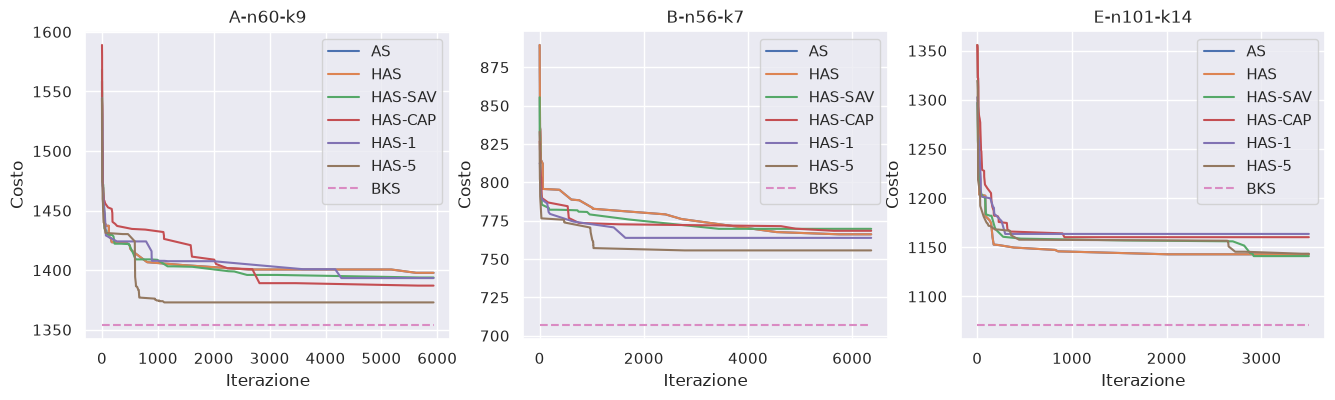
\includegraphics[width=1.0\linewidth]{output.png}
    \caption{Curve di convergenza delle istanze A-n60-k9, B-n56-k7, E-n101-k14.}
    \label{fig:curves}
\end{figure}

\noindent
È stato scelto di approfondire l'analisi delle istanze \textit{A-n60-k9}, \textit{B-n56-k7}, \textit{E-n101-k14}. Le curve di convergenza sono mostrate in \autoref{fig:curves}, per ogni istanza del problema sono stati messi a confronto i vari profili, ad eccezione di \textit{NN}, la linea tratteggiata color porpora rappresenta la \textit{Known Best Solution} dell'istanza.
\begin{figure}[H]
    \centering
    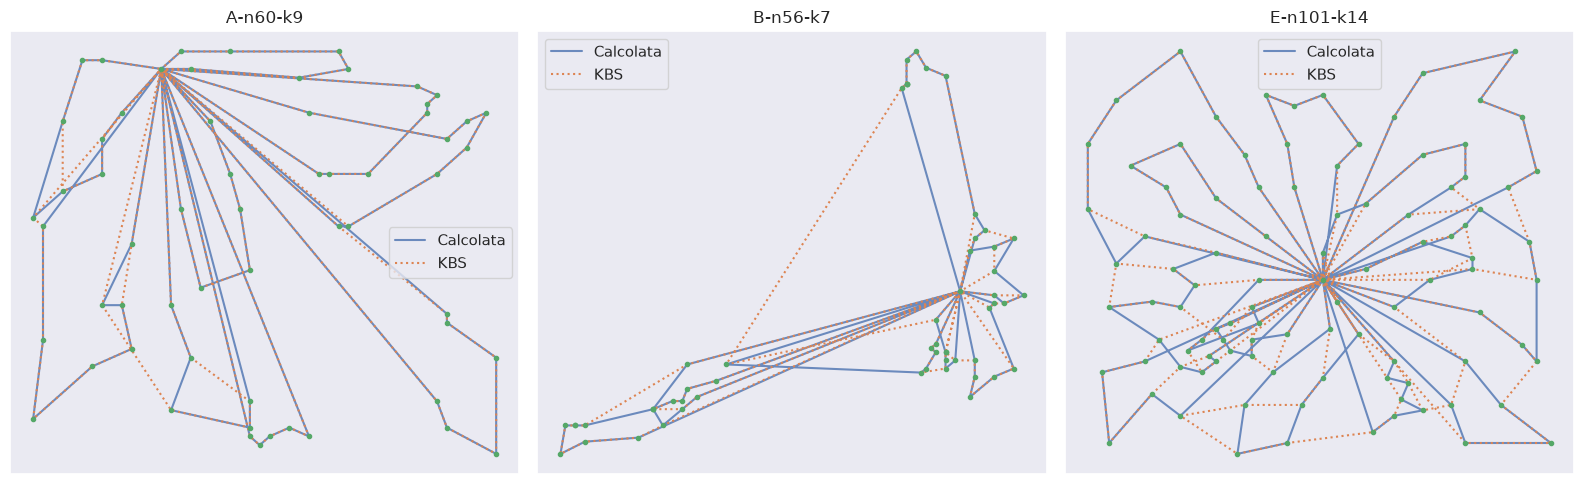
\includegraphics[width=1\linewidth]{plots.png}
    \caption{Soluzioni migliori delle istanze A-n60-k9, B-n56-k7, E-n101-k14.}
    \label{fig:comparisons}
\end{figure}

L'algoritmo generalmente produce buoni risultati con un basso numero di iterazioni: il profilo \textit{HAS-5} converge molto rapidamente nelle prime due istanze, dove le successive iterazioni generalmente non riconducono a risultati migliori; mentre nella terza, \textit{HAS} e \textit{AS} hanno una convergenza più rapida, con \textit{HAS-5} e \textit{HAS-SAV} che migliorano significativamente nelle ultime \(1000\) iterazioni, e quest'ultimo profilo produce un risultato marginalmente migliore. In \autoref{fig:comparisons}  sono confrontati i percorsi ottenuti con i percorsi della soluzione migliore, è immediato notare come nelle prime istanze i nodi sono generalmente clusterizzati ( molto evidente nella seconda ), mentre nella terza i nodi sono distribuiti più uniformemente e il deposito è localizzato in posizione centrale.

\section{Conclusioni}
Il presente progetto ha permesso la realizzazione di un algoritmo \textit{Ant Colony Optimization} per risolvere il problema del \textit{Capacited Vehicle Routing Problem}, basandosi su proposte e risultati della letteratura scientifica esistente. Dove possibile, è stato scelto di combinare diverse strategie: alcune intrinseche all'algoritmo, come le misure si risparmio e capacità, la \textit{MAX-MIN Ant System}; altre implementative, come il \textit{Log-Sum-Exp trick} e il calcolo multi processore con la libreria \textit{multiprocessing}.
\\La metodologia di lavoro ha privilegiato la realizzazione dell'algoritmo di risoluzione per il problema assegnato, a discapito della ricerca esaustiva dei parametri, ottenendo comunque buoni risultati con i profili suggeriti dalla letteratura \cite{Bullnheimer}.
\subsection{Sviluppi Futuri}
Nonostante i buoni risultati ottenuti e la solidità dell'implementazione prodotta, si suggeriscono eventuali evoluzioni:
\begin{itemize}
    \item Una più \textbf{estesa esplorazione dei parametri}  in particolare il fine-tuning del parametro di evaporazione $\rho$  e l'influenza del feromone $\alpha$, studiare l'influenza dello \textit{smoothing} del feromone\cite{STUTZLE2000889} nei risultati, parametro non utilizzato nella sperimentazione. Inoltre l'\textbf{introduzione di nuove euristiche} per la ricerca locale alternativi al \textit{2-Opt}, come il \textit{3-Opt} o l'\textit{algoritmo Kernighan–Lin}, potrebbe significativamente migliorare la qualità delle soluzioni.
    \item \textbf{Migliorare i tempi di esecuzione} è di vitale importanza per supportare l'attività di ricerca dei parametri e il calcolo di soluzioni, pertanto si suggerisce di esplorare un \textbf{approccio vettorizzato} all'algoritmo, che sfrutti quanto il più possibile le istruzioni SIMD dei processori, offerti già trasparentemente da \textit{numpy} per molte operazioni sui tipi della libreria: una tale evoluzione, inoltre, renderebbe triviale adattare il codice per essere eseguito su unità di calcolo massivamente parallele, come le GPU.
\end{itemize}



\printbibliography %Prints bibliography
\end{document}
